\section{Design of the equalizer}
This chapter aims to describe the design of an digital graphic equalizer, for an electric guitar. By graphic equalizer it is meant that only the gain of each band is changeable for the user.  
To begin with, some design choices have to made. From \autoref{tab:frequency_area} it is seen that the frequency area of an electric guitar is from \SI{80}{\hertz} to \SI{4400}{\hertz}. Thus the equalizer has to be able to change the frequency response in this area. This change in the frequency response is made by a combination of shelving filters and peak filters. The shelving filters are used for the highest and the lowest bands of the equalizer and the peak filters are used for the in between bands. All filters are normally kept as first or second order filters. 

\subsection{Shelving filter}
The transfer function for a first order low shelving filter is as in \autoref{eq:analog_shelving_low} \citep{Julius_smith}.

\begin{equation}\label{eq:analog_shelving_low}
        H_{LS}(s) = G \cdot \frac{\omega_c}{s+\omega_c}
    \end{equation}

    \startexplain
    \explain{$H_{LS}(s)$ is the low shelving filters transfer function.}{\si{1}}
     \explain{$G$ is the gain.}{\si{1}}
	\explain{$\omega_c$ is the transition frequency dividing low and high frequencies.}{\si{\radian/\second}}
    \stopexplain
    
The transfer function for a first order high shelving filter is as in \autoref{eq:analog_shelving_low}.

\begin{equation}\label{eq:analog_shelving_high}
        H_{HS}(s) = G \cdot \frac{s}{s+\omega_c}
    \end{equation}

    \startexplain
    \explain{$H_{HS}(s)$ is the high shelving filters transfer function.}{\si{1}} 
    \stopexplain

    
When implementing \autoref{eq:analog_shelving_low} and \autoref{eq:analog_shelving_high}, individually in a feedforward loop, as in \autoref{fig:shelving_block}, the bodeplots of first order low- and high- shelving filters with different cut-off frequencies, becomes as in \autoref{fig:low_and_high_shelving}.

\begin{figure}[!h]
\centering
\def\svgwidth{0.72\columnwidth}
\scalebox{1}{\input{figures/design/shelving_filter_block.pdf_tex}}
\caption{Block diagram of the shelving filter.}
		\label{fig:shelving_block}
\end{figure}

\begin{figure}
    \centering
        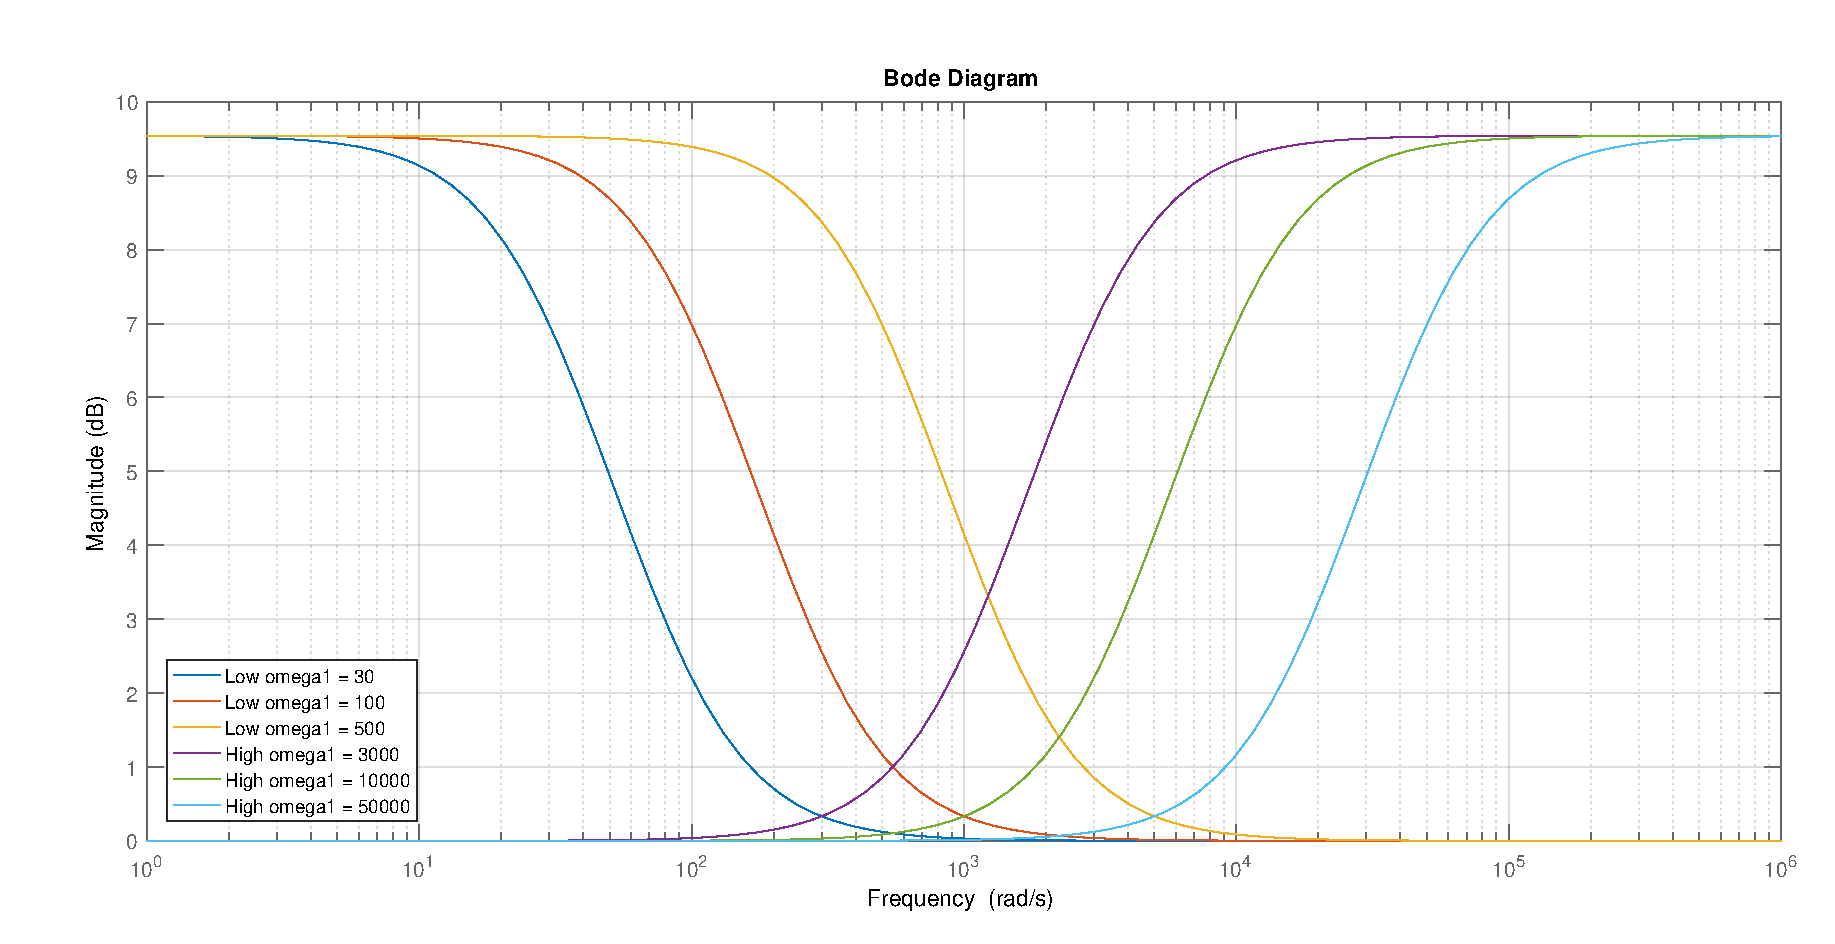
\includegraphics[width=\textwidth]{low_and_high_shelfing.pdf}
        \caption{Bodeplot of first order low- and high- shelving filters with different transition frequencies.}
        \label{fig:low_and_high_shelving}
  \end{figure} 
  %\todo[inline]{figure is now first order}

\subsection{Peak filter}
The peak filters for the in between bands can be made from a number of design topologies. One of these are the constant-Q design. This design is sufficient the way that it keeps a specified bandwidth of the filter and therefore each individual filter's impact on the neighbouring filters can be controlled \citep{constant_Q}.
A way to make these constant-Q peak filters, and keep the order of the filter low, is by combining a second order lowpass filter with a high Q-value, and a linear function in Laplace domain.
The transfer function for the analog second order lowpass filter is as in \autoref{eq:analog_2nd_order_LP} and the transfer function for the analog linear function is as in \autoref{eq:analog_linear_function}. Their bodeplot can be seen in \autoref{fig:lin_function_&_2nd_order_LP}, where $Q = 4$ and $\omega_0 = 1000$. 

\begin{equation}\label{eq:analog_2nd_order_LP}
        H_{LP}(s) = \frac{\omega_0^2}{s^2+\frac{\omega_0}{Q}\cdot s + \omega_0^2}
    \end{equation}

    \startexplain
     \explain{$\omega_0$ is the cut-off frequency.}{\si{\radian/\second}}
     \explain{$Q$ is the ratio between the center frequency and the bandwidth.}{\si{1}}
    \stopexplain

\begin{equation}\label{eq:analog_linear_function}
        H_{lin}(s) = \frac{s}{\omega_0 \cdot Q}
    \end{equation}
    
\begin{figure}
    \centering
        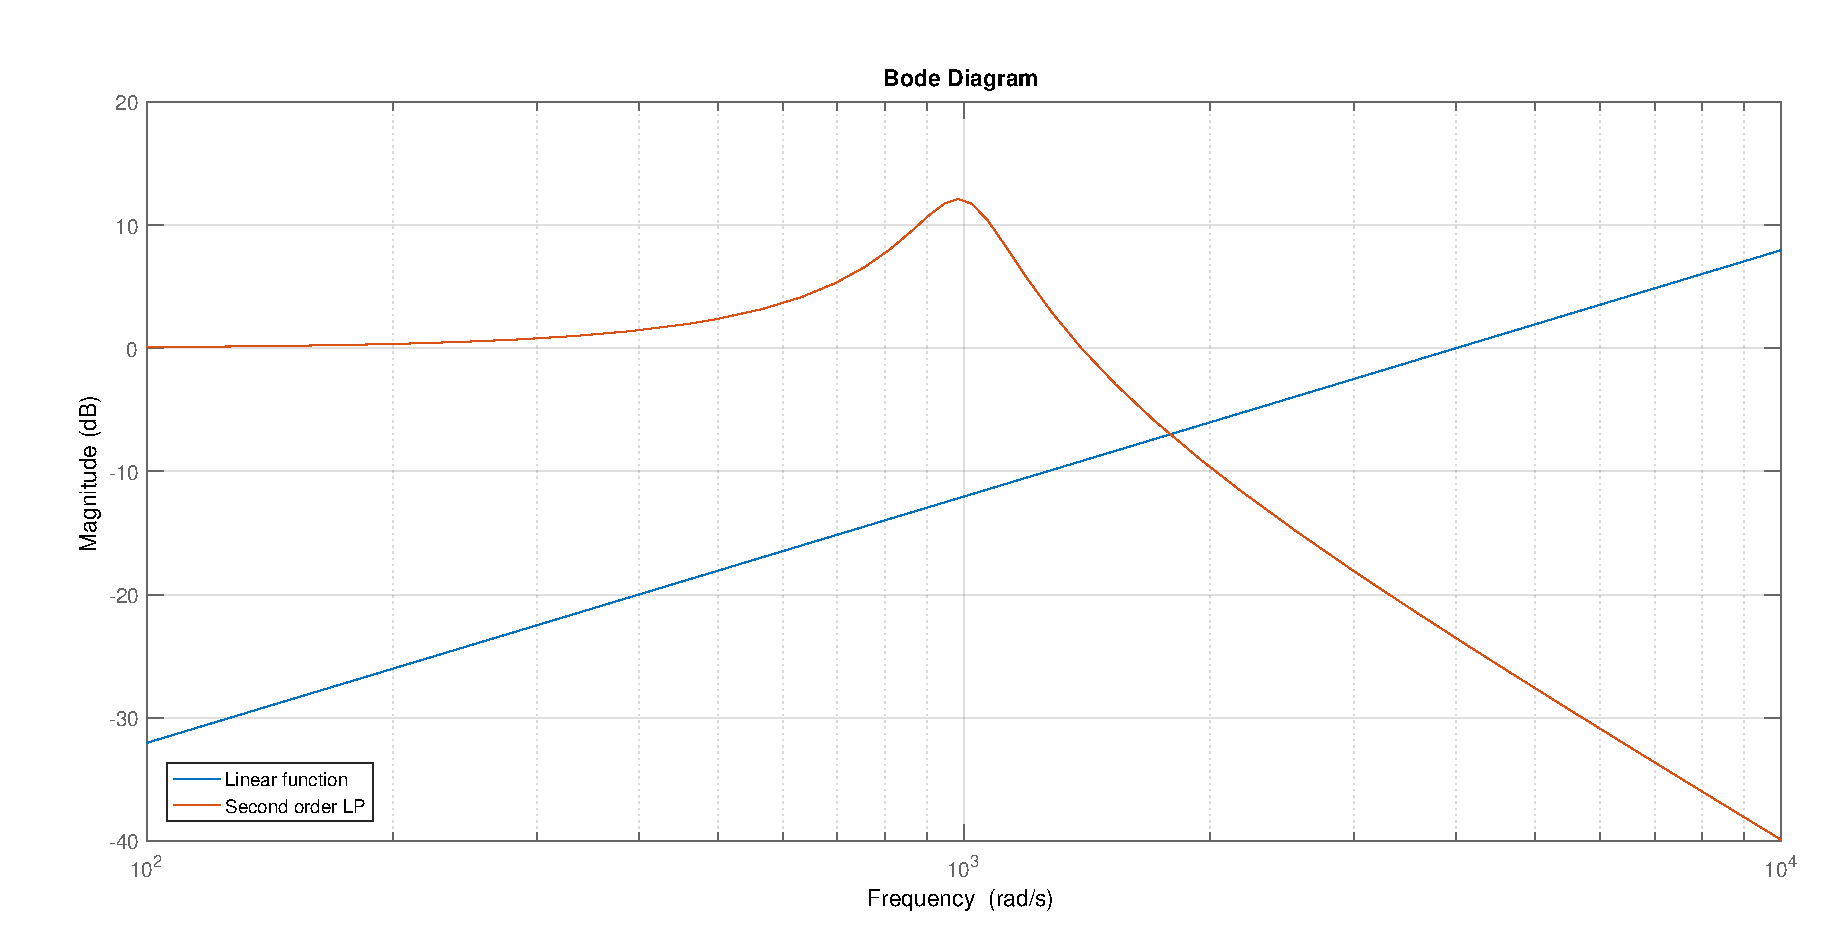
\includegraphics[width=\textwidth]{linear_function_and_2nd_order_LP.pdf}
        \caption{Bodeplot of a linear function and second order lowpass filter.}
        \label{fig:lin_function_&_2nd_order_LP}
  \end{figure} 

To make a peak filter, the two functions in \autoref{fig:lin_function_&_2nd_order_LP} are connected in series to make the analog peak filter transferfuntion as in \autoref{eq:H_peak}.

\begin{equation}\label{eq:H_peak}
        H_{peak}(s) = G \cdot \frac{\frac{\omega_0}{Q}\cdot s}{s^2+\frac{\omega_0}{Q}\cdot s + \omega_0^2}
    \end{equation}
    
    \startexplain
    \explain{$H_{peak}(s)$ the analog transferfunction of the peak filter.}{\si{1}}
     \explain{$G$ is the gain of the peak filter.}{\si{1}}
    \stopexplain

\begin{figure}[!h]
\centering
\def\svgwidth{\columnwidth}
\input{figures/design/peak_filter_block.pdf_tex}
\caption{Block diagram of a peak filter.}
		\label{fig:peak_filter_block}
\end{figure}

When implementing \autoref{eq:H_peak} in a feedforward loop as in \autoref{fig:peak_filter_block}, the bodeplot becomes as in \autoref{fig:peak_filter}, where $Q = 4$, $\omega_0 = 1000$ and various gain values. 



\begin{figure}[!h]
    \centering
        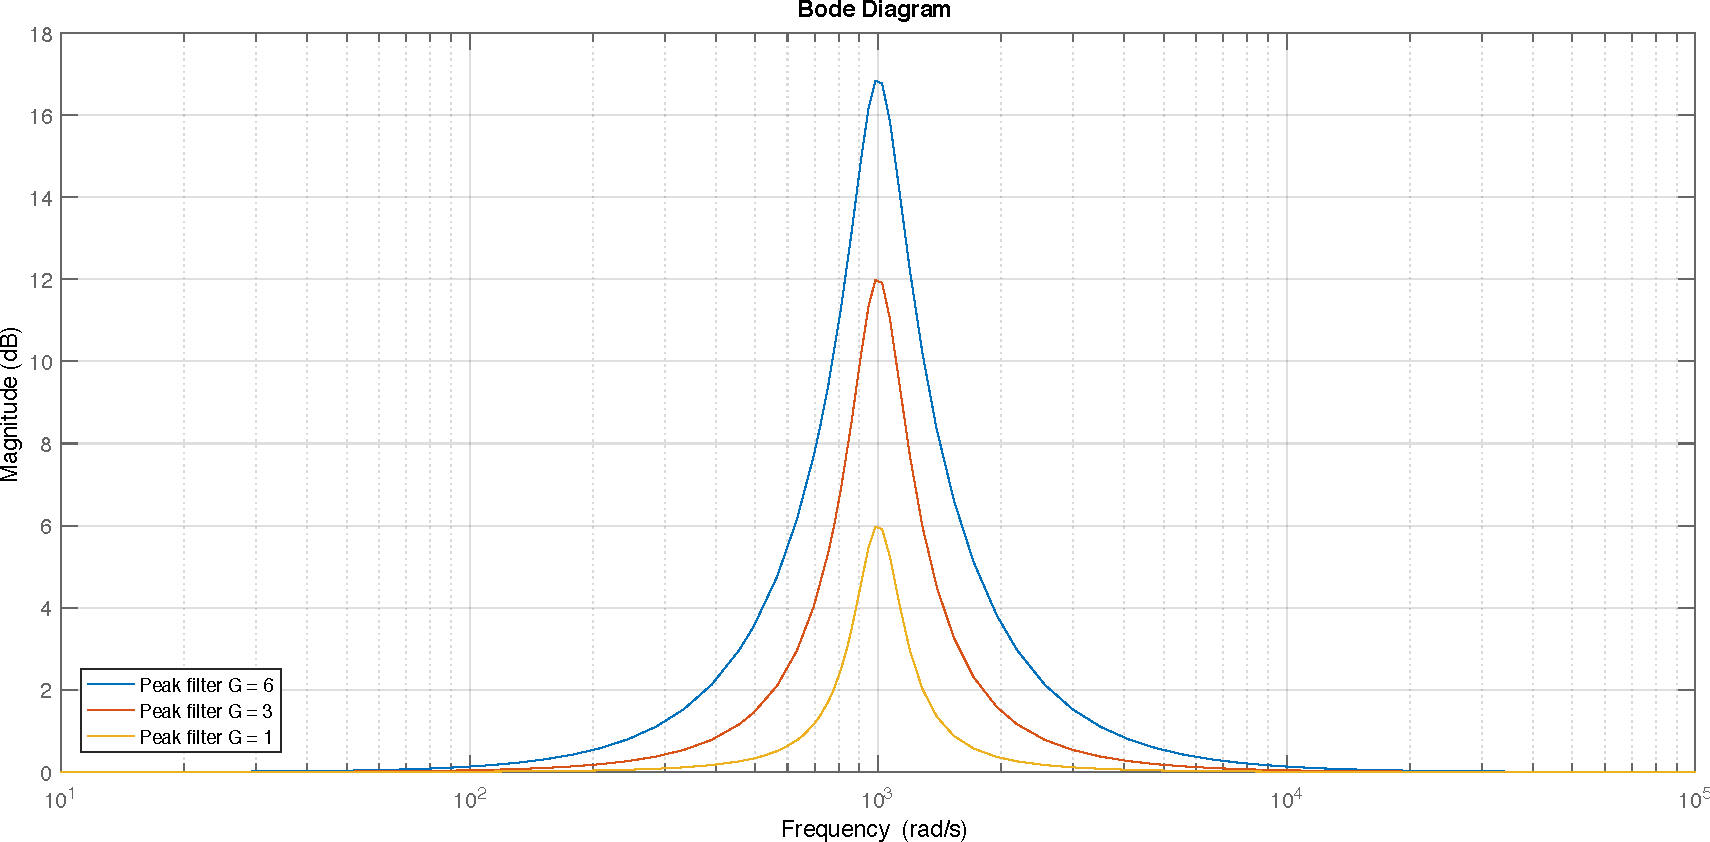
\includegraphics[width=\textwidth]{peak_filter.pdf}
        \caption{Bodeplot of a peak filter with various gain values.}
        \label{fig:peak_filter}
  \end{figure} 
  
\subsection{Design choices and calculation of filter parameters}
All the parts needed to make an equalizer have now been described. The parameters after which the equalizer shall be designed, will now be presented. 
The equalizer will be inspired by the BOSS GE-7 which is an analog equalizer for an electric guitar. The equalizer designed in this report will have the same number of bands and have the same attenuation and amplification ranges as the BOSS GE-7 \citep{Boss_GE7}. Thus the equalizer will have seven bands and be able to amplify each band $\pm$ \SI{15}{\decibel}.
The center frequencies of the seven bands are also inspired by the BOSS GE-7 and is placed as in \autoref{tab:center_frequencies}.

\begin{table}[htbp]
\centering
\caption{Center frequencies for the equalizer.}
\label{tab:center_frequencies}
\begin{tabular}{|l|l|}
\cline{1-2}
\textbf{Band} & \textbf{Center frequency} \\ \cline{1-2}
1st & \SI{100}{\hertz} \\  \cline{1-2}
2nd & \SI{200}{\hertz}\\ \cline{1-2}
3rd & \SI{400}{\hertz} \\ \cline{1-2}
4th & \SI{800}{\hertz} \\ \cline{1-2}
5th & \SI{1600}{\hertz} \\ \cline{1-2}
6th & \SI{3200}{\hertz} \\ \cline{1-2}
7th & \SI{6400}{\hertz} \\ \cline{1-2}
\end{tabular}
\end{table}

The first and the seventh band will be made by shelving filters and band 2,3,4,5 and 6 will be made by peak filters. The aim of the design is to design an equalizer, where each band can be amplified $\pm$ \SI{15}{\decibel} and has a flat combined frequency response when each band is set to amplify \SI{15}{\decibel}.
The individual filters in the amplifying equalizer will coupled in parallel as seen in \autoref{fig:eq_parallel}.

\begin{figure}[!h]
\centering
\def\svgwidth{0.72\columnwidth}
\scalebox{1}{\input{figures/design/eq_parallel.pdf_tex}}
\caption{Block diagram of the combined amplifying equalizer.}
		\label{fig:eq_parallel}
\end{figure}

The shelving filters will be designed first, followed by the peak filters. Since the transition frequencies, $\omega_c$ for the low- filter and high shelving filters, are found in \autoref{tab:center_frequencies}, the only unknown in \autoref{eq:analog_shelving_low} is the gain, $G$.
The gain has to be changeable within $\pm$ \SI{15}{\decibel}. It is chosen that it is the passband that will be amplified \SI{15}{\decibel} and not the transition frequency, $\omega_c$. Thus the shelving filters gain is found by setting $\omega_c =$ \SI{100}{\radian/\second} and then finding the gain for $\omega =$ \SI{1}{\radian/\second}. The gain value for a \SI{15}{\decibel} attenuation is found in \autoref{eq:shelving_gain_value}.

\begin{subequations}
\begin{equation}\label{eq:shelving_gain}
       20 \cdot \log_{10} \left( \mathopen|1 + H_{LS}(j\cdot \omega) \mathclose| \right) = 15 \addunit{\SI{}{\decibel}}
    \end{equation}
 \centering
$\Updownarrow$   
\begin{equation}\label{eq:shelving_gain_value}
       G_{LS-boost} = \frac{\sqrt{(\omega_c^2+\omega^2) \cdot 10^{\frac{12}{10}}-\omega^2}}{\omega_c} - 1 \Big|_{\omega = 1 \ and \ \omega_c = 100} = 4.62 \addunit{\SI{}{1}}
    \end{equation}
\end{subequations}

All parameters in the shelving filters are now known and the peak filters will now be designed.
Since $\omega_0$ is fixed for each band, only $G$ and $Q$ have to be determined. The gain, $G$, has to changeable within $\pm$ \SI{15}{\decibel}.
What the gain should be for the band to amplify \SI{15}{\decibel} is found in \autoref{eq:peak_gain_value}


\begin{subequations}
\begin{equation}\label{eq:peak_gain}
       20 \cdot \log_{10} \left(\mathopen|1 + H_{peak}(j\omega_0)\mathclose|\right) = 20 \cdot \log_{10} \left(1+G_{peak-boost}\right) = 15 \addunit{\SI{}{\decibel}}
    \end{equation}
\centering
$\Updownarrow$
\begin{equation}\label{eq:peak_gain_value}
        G_{peak-boost} = -1+10^{\frac{3}{4}} = 4.62 \addunit{\SI{}{1}}
    \end{equation}
 \end{subequations}
 
 

The Q-value is then the only unknown in the design of the peak filters. In \autoref{req:equalizer2} it is stated that at full amplification (\SI{15}{\decibel}), the amplification at the neighbouring centerfrequencies must drop to (\SI{9}{\decibel}). 
The Q-value will be chosen so it has the minimum ripple. This Q-value is found using a MATLAB program, where the Q-value is increased in steps of 0.2 from 0 to 10. All gains on both the peak and the shelving filters are set to amplify \SI{15}{\decibel}. The optimal Q-value is hereby found to be 1.4, giving a ripple of $\pm$\SI{1.11}{\decibel}, in the frequency area from \SI{100}{\hertz} to \SI{6400}{\hertz}, when all filters are fully amplified. All parameters for the peak filters are then found. 
When coupling the filters as in \autoref{fig:eq_parallel}, and plotting it in MATLAB, the bodeblot of the equalizer with all filters fully amplified, is as in \autoref{fig:eq_s_domain_comb}. In the figure all bands have their maximum gain value.

\begin{figure}[!h]
    \centering
        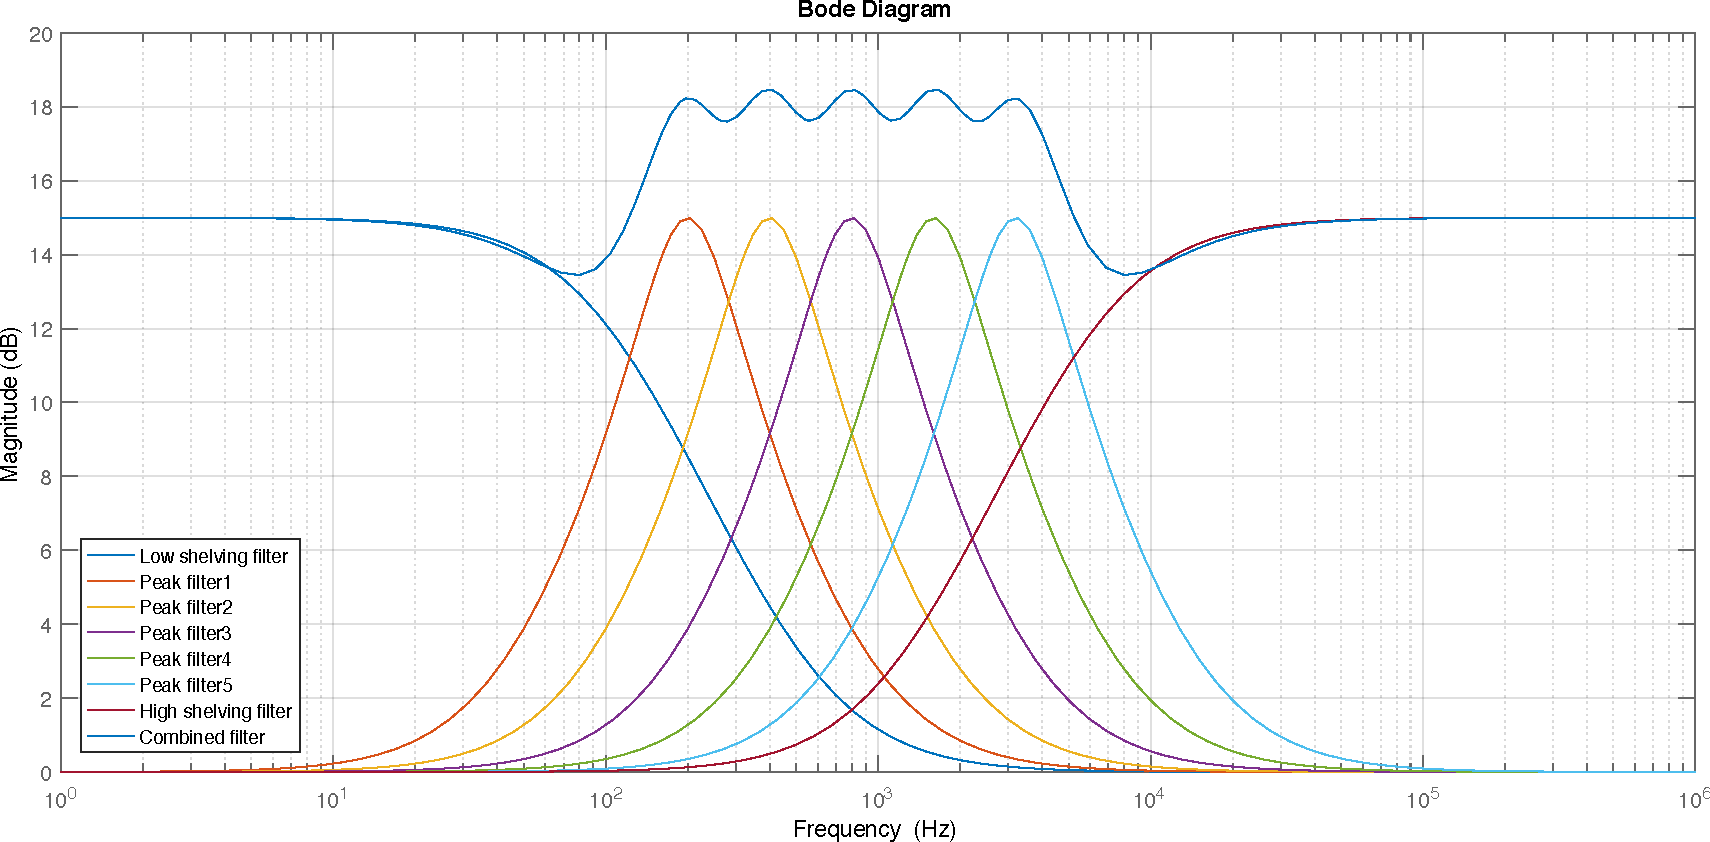
\includegraphics[width=\textwidth]{eq_s_domain_comb.pdf}
        \caption{Bodeplot of the combined equalizer in s-domain, with maximum gain on all bands.}
        \label{fig:eq_s_domain_comb}
  \end{figure}

The ripple of the combined equalizer in s-domain, when all bands are fully amplified, is \SI{4.49}{\decibel}, in the frequency area from \SI{100}{\hertz} to \SI{6400}{\hertz}. This ripple is accepted as a compromise, in order to make each band independent from the neighbouring bands. 

It is chosen that the equalizer shall be able to amplify each band in five different steps from \SI{0}{\decibel} to \SI{15}{\decibel}. Using \autoref{eq:shelving_gain} and \autoref{eq:peak_gain}, and changing the value on the right side of the equality sign, the gain values for the five steps are found. The gain values are shown in \autoref{tab:eq_gain_values}. 

\begin{table}[htbp]
\centering
\caption{Gain values for the equalizer.}
\label{tab:eq_gain_values}
\begin{tabular}{|l|l|l|}
\cline{1-3}
\textbf{Amplification [dB]} & \textbf{Gain value (shelving)} & \textbf{Gain value (peak)} \\ \cline{1-3} 
3 & 0.41 & 0.41 \\  \cline{1-3} 
6 & 0.99 & 0.99 \\ \cline{1-3} 
9 & 1.81 & 1.81 \\ \cline{1-3} 
12 & 2.98 & 2.98 \\ \cline{1-3} 
15 & 4.62 & 4.62 \\ \cline{1-3} 
\end{tabular}
\end{table}

\subsection{Converting the equalizer to z-domain}
In order to implement the equalizer on a \gls{dsp}, the now designed analog equalizer, has be to converted to a digital equalizer. This conversion will be made by using the bilinear transformation, which converts analog filters into digital IIR filters. In \autoref{eq:bilinear_transformation} the bilinear transformation method is shown.

\begin{equation}\label{eq:bilinear_transformation}
        H(z) = H(s) \Big|_{s = \frac{2}{T_s} \cdot \frac{z-1}{z+1}}
    \end{equation}
    
    \startexplain
     \explain{$H(z)$ is the digital transferfunction.}{\si{1}}
     \explain{$T_s$ is the sample time.}{\si{\second}}
    \stopexplain
    
Applying this conversion on the shelving and the peak filters, the digital transferfunctions becomes as in \autoref{eq:Hz_LS}, \autoref{eq:Hz_HS} and \autoref{eq:H_peak}.

\begin{equation}\label{eq:Hz_LS}
        H(z)_{LS} = G \cdot \frac{z \cdot a_{LS1} + a_{LS2}}{z \cdot b_{LS1} + b_{LS2}}
    \end{equation}
    
    \startexplain
     \explain{$H(z)_{LS}$ is the digital transferfunction for the low shelving filter.}{\si{1}}
     \explain{$a_{LS1} = a_{LS2} = \omega_c \cdot T_s$ }{\si{1}}
     \explain{$b_{LS1} = 2+\omega_c \cdot T_s$ }{\si{1}}
     \explain{$b_{LS2} = -2+\omega_c \cdot T_s$ }{\si{1}}
    \stopexplain
    
\begin{equation}\label{eq:Hz_HS}
        H(z)_{HS} = G \cdot \frac{z \cdot a_{HS1} + a_{HS2}}{z \cdot b_{HS1} + b_{HS2}}
    \end{equation}
    
    \startexplain
     \explain{$H(z)_{HS}$ is the digital transferfunction for the high shelving filter.}{\si{1}}
     \explain{$a_{HS1} = 2$ }{\si{1}}
     \explain{$a_{HS2} = -2$ }{\si{1}}
     \explain{$b_{HS1} = 2+\omega_c \cdot T_s$ }{\si{1}}
     \explain{$b_{HS2} = -2+\omega_c \cdot T_s$ }{\si{1}}
    \stopexplain

\begin{equation}\label{eq:Hz_peak}
        H(z)_{peak} = G \cdot \frac{z^2 \cdot a_{peak1} + a_{peak2}}{z^2 \cdot b_{peak1} + z \cdot b_{peak2} + b_{peak3}}
    \end{equation}
    
    \startexplain
     \explain{$H(z)_{peak}$ is the digital transferfunction for the peak filter.}{\si{1}}
     \explain{$a_{peak1} = 2 \cdot \omega_0 \cdot T_s$ }{\si{1}}
     \explain{$a_{peak2} = -2 \cdot \omega_0 \cdot T_s$ }{\si{1}}
     \explain{$b_{peak1} = 4 \cdot Q + 2 \cdot \omega_c \cdot T_s + \omega_0^2 \cdot T_s^2 \cdot Q$ }{\si{1}}
     \explain{$b_{peak2} = -8 \cdot Q + 2 \cdot  \omega_0^2 \cdot T_s^2 \cdot Q$ }{\si{1}}
     \explain{$b_{peak3} = 4 \cdot Q - 2 \cdot \omega_c \cdot T_s + \omega_0^2 \cdot T_s^2 \cdot Q$ }{\si{1}}
    \stopexplain

The combined transferfunction, when combining the transferfunctions as in \autoref{fig:eq_parallel}, becomes as in \autoref{fig:eq_z_domain_comb}.

\begin{equation}\label{eq:z_to_n_final}
        H(z)_{comb} = 1 + H(z)_{LS} + H(z)_{HS} +  \sum_{j=1}^{5} H(z)_{peak(j)}
    \end{equation}

When choosing the sampling frequency, $f_s =$ \SI{44.1}{\kilo \hertz}, and thereby $T_s = \frac{1}{f_s} =$ \SI{22.68}{\micro \second}, setting $Q = 1.4$, and using the frequencies in \autoref{tab:center_frequencies} as $\omega_c$ and $\omega_0$, the frequency response of the digital equalizer, with all bands fully amplified, looks like in \autoref{fig:eq_z_domain_comb}.

\begin{figure}[!h]
    \centering
        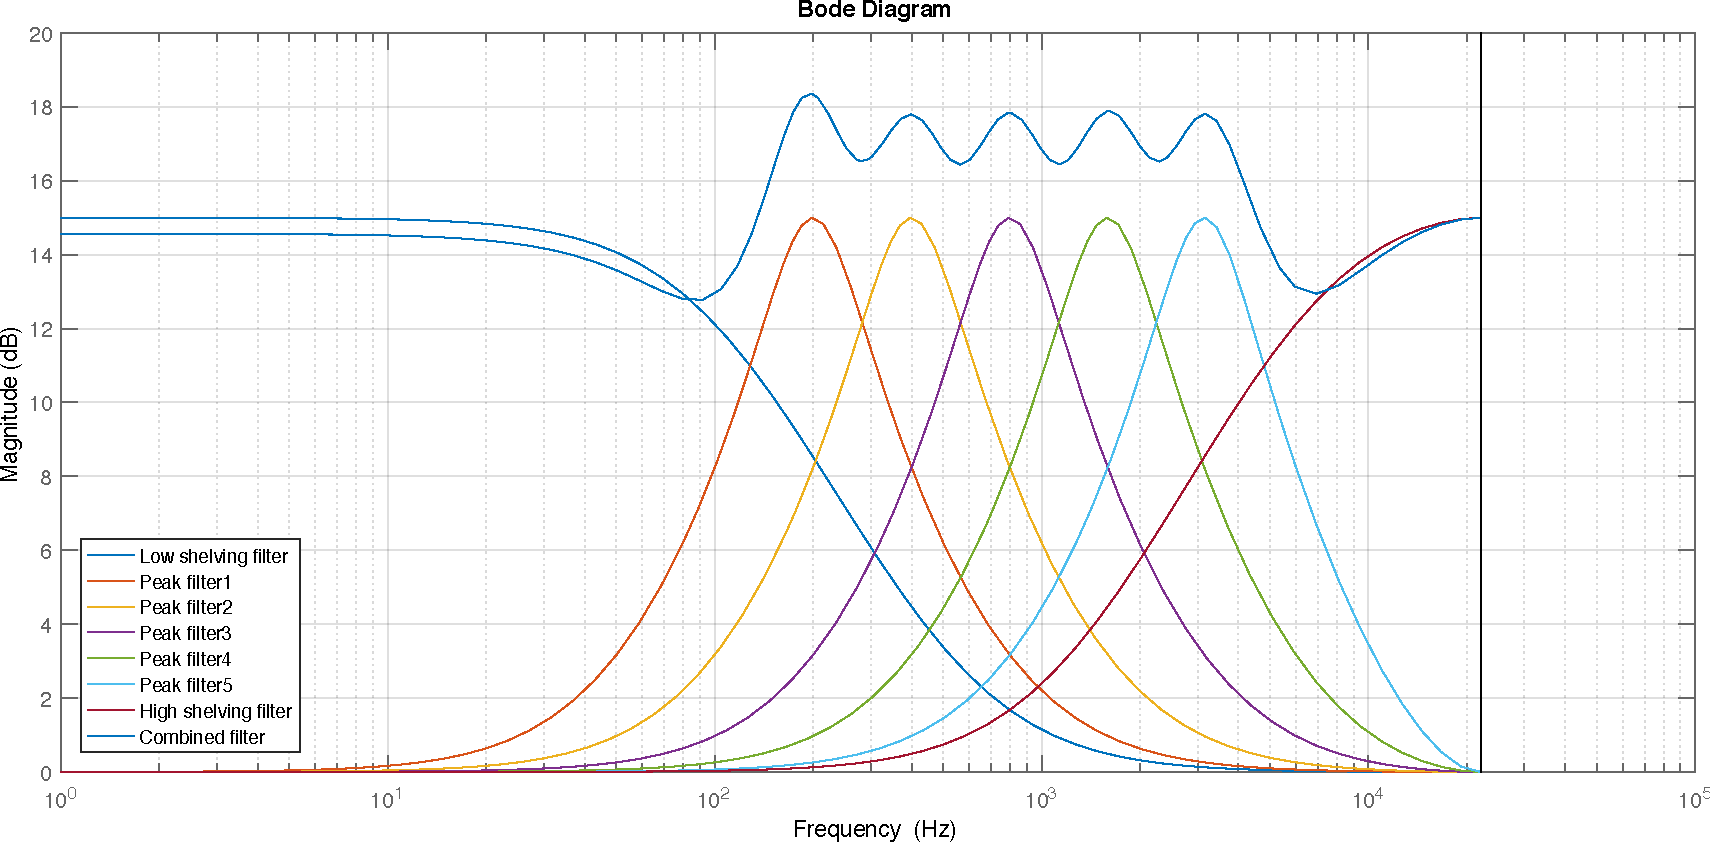
\includegraphics[width=\textwidth]{eq_z_domain_comb.pdf}
        \caption{Bodeplot of the combined equalizer in z-domain, with maximum gain on all bands.}
        \label{fig:eq_z_domain_comb}
  \end{figure}

The conversion is made without prewarping, because the frequency response, when using prewarping, changed in an unwanted way at low frequencies.

\subsection{Converting the equalizer to n-domain}
The last step in making the equalizer implementable in a \gls{dsp}, is to convert the z-domain transferfunction, into a differential equation in n-domain. The procedure of doing this, will be shown for the peak filters, but the procedure is the same for the shelving filters. The conversion from z-domain to n-domain is shown in the equations \autoref{eq:z_to_n1} to \autoref{eq:z_to_n7} 

\begin{subequations}
\begin{equation}\label{eq:z_to_n1}
       H(z)_{peak} = \frac{Y(z)}{X(z)} = G \cdot \frac{z^2 \cdot a_{peak1} + a_{peak2}}{z^2 \cdot b_{peak1} + z \cdot b_{peak2} + b_{peak3}}
    \end{equation}

\begin{equation}\label{eq:z_to_n2}
        \frac{Y(z)}{X(z)} = G \cdot \frac{a_{peak1} + a_{peak2} \cdot z^{-2}}{b_{peak1} + b_{peak2} \cdot z^{-1} + b_{peak3} \cdot z^{-2}}
    \end{equation}
    \centering
$\Updownarrow$
\begin{equation}\label{eq:z_to_n3}
        Y(z) \cdot (b_{peak1} + b_{peak2} \cdot z^{-1} + b_{peak3} \cdot z^{-2}) = X(z) \cdot G \cdot (a_{peak1} + a_{peak2} \cdot z^{-2})
    \end{equation}
       \centering
$\Updownarrow$
\begin{equation}\label{eq:z_to_n4}
         Y(z) \cdot b_{peak1} + Y(z) \cdot b_{peak2} \cdot z^{-1} + Y(z) \cdot b_{peak3} \cdot z^{-2} =  G \cdot (X(z) \cdot a_{peak1} + X(z) \cdot a_{peak2} \cdot z^{-1})
    \end{equation}
    \centering
    $\Downarrow Z^{-1}$
\begin{equation}\label{eq:z_to_n5}
         b_{peak1} \cdot y[n] + b_{peak2} \cdot y[n-1] + b_{peak3} \cdot y[n-2] =  G \cdot (a_{peak1} \cdot x[n] + a_{peak2} \cdot x[n-2])
    \end{equation}
    \centering
    $\Updownarrow$
\begin{equation}\label{eq:z_to_n6}
         b_{peak1} \cdot y[n] =  G \cdot (a_{peak1} \cdot x[n] + a_{peak2} \cdot x[n-2]) -  b_{peak2} \cdot y[n-1] - b_{peak3} \cdot y[n-2]
    \end{equation}
    \centering
    $\Updownarrow$
\begin{equation}\label{eq:z_to_n7}
         y_{peak}[n] = \frac{G \cdot a_{peak1}}{b_{peak1}} \cdot x[n] + \frac{G \cdot a_{peak2}}{b_{peak1}} \cdot x[n-2] -  \frac{b_{peak2}}{b_{peak1}} \cdot y_{peak}[n-1] - \frac{b_{peak3}}{b_{peak1}} \cdot y_{peak}[n-2]
    \end{equation}
    
    \startexplain
     \explain{$y[n]$ is the output sample.}{\si{1}}
     \explain{$x[n]$ is the input sample.}{\si{1}}
    \stopexplain
 \end{subequations}
 

\autoref{eq:z_to_n7} is the differential equation which is ready to be implemented digitally. When following the same procedure for the low shelving filter and the high shelving filter, their differential equations become as in \autoref{eq:z_to_n_LS} and \autoref{eq:z_to_n_HS}.

\begin{equation}\label{eq:z_to_n_LS}
        y_{LS}[n] = \frac{G \cdot a_{LS1}}{b_{LS1}} \cdot x[n] + \frac{G \cdot a_{LS2}}{b_{LS1}} \cdot x[n-1] -  \frac{b_{LS2}}{b_{LS1}} \cdot y_{LS}[n-1]
    \end{equation}

\begin{equation}\label{eq:z_to_n_HS}
        y_{HS}[n] = \frac{G \cdot a_{HS1}}{b_{HS1}} \cdot x[n] + \frac{G \cdot a_{HS2}}{b_{HS1}} \cdot x[n-1] -  \frac{b_{HS2}}{b_{HS1}} \cdot y_{HS}[n-1]
    \end{equation}

When coupling the filters as in \autoref{fig:eq_parallel}, the combined output of the equalizer becomes as in \autoref{eq:z_to_n_final}.

\begin{equation}\label{eq:z_to_n_final}
        y_{comb}[n] = x[n] + y_{LS}[n] + y_{HS}[n] + \sum_{j=1}^{5} y_{peak(j)}[n]
    \end{equation}

It is now possible for the equalizer to amplify different frequency areas.

\subsection{The inverse equalizer}
The attenuating part of the equalizer will be made from a series connection of feedback loops. The initial idea was to implement the attenuating part as a parallel connection of feedback loops, where the differential equations from the amplifying part could be reused. The initial idea was changed because of problems when inverting the parallel feedback connection. 
The attenuating part will be implemented as illustrated in \autoref{fig:eq_attenuate_block}.

\begin{figure}[!h]
\centering
\def\svgwidth{0.72\columnwidth}
\scalebox{1}{\input{figures/design/eq_attenuate_block.pdf_tex}}
\caption{Block diagram of the attenuating equalizer.}
		\label{fig:eq_attenuate_block}
\end{figure}

The differential equations for each feedback loop are derived by the same method as for the amplifying part, but with different analog transferfunctions. The attenuating analog transferfunction reuse the amplifying analog transferfunction, but in as a feedback loop, as shown in \autoref{eq:analog_attenuate}.

\begin{equation}\label{eq:analog_attenuate}
        H_{cut}(s) = \frac{1}{1 + H_{boost}}
    \end{equation}
    
    \startexplain
     \explain{$H_{cut}(s)$ is the attenuating transferfunction.}{\si{1}}
     \explain{$H_{boost}$ can be either $H_{LS}(s)$, $H_{HS}(s)$ or $H_{peak}(s)$.}{\si{1}}
    \stopexplain
    
The three new transferfunctions from \autoref{eq:analog_attenuate} are bilinear transformed and converted from z-domain to n-domain, the same way as the amplifying part. The z-domain transferfunctions for the attenuating low shelving-, high shelving- and peak filter, are shown in \autoref{eq:Hz_LS_att}, \autoref{eq:Hz_HS_att} and \autoref{eq:Hz_peak_att}.

\begin{equation}\label{eq:Hz_LS_att}
        H(z)_{LS-cut} =\frac{z \cdot a_{LS1-cut} + a_{LS2-cut}}{z \cdot b_{LS1-cut} + b_{LS2-cut}}
    \end{equation}
    
    \startexplain
     \explain{$H(z)_{LS-cut}$ is the digital transferfunction for the attenuating low shelving filter.}{\si{1}}
     \explain{$b_{LS1-cut} = G \cdot T_s \cdot \omega_c + T_s \cdot \omega_c +2$ }{\si{1}}
     \explain{$b_{LS2-cut} = G \cdot T_s \cdot \omega_c + T_s \cdot \omega_c -2$ }{\si{1}}
     \explain{$a_{LS1-cut} = 2+\omega_c \cdot T_s$ }{\si{1}}
     \explain{$a_{LS2-cut} = -2+\omega_c \cdot T_s$ }{\si{1}}
    \stopexplain
    
\begin{equation}\label{eq:Hz_HS_att}
        H(z)_{HS-cut} = \frac{z \cdot a_{HS1-cut} + a_{HS2-cut}}{z \cdot b_{HS1-cut} + b_{HS2-cut}}
    \end{equation}
    
    \startexplain
     \explain{$H(z)_{HS-cut}$ is the digital transferfunction for the attenuating high shelving filter.}{\si{1}}
     \explain{$b_{HS1-cut} = T_s \cdot \omega_c + 2 \cdot G +2$ }{\si{1}}
     \explain{$b_{HS2-cut} = T_s \cdot \omega_c - 2 \cdot G -2$ }{\si{1}}
     \explain{$a_{HS1-cut} = 2+\omega_c \cdot T_s$ }{\si{1}}
     \explain{$a_{HS2-cut} = -2+\omega_c \cdot T_s$ }{\si{1}}
    \stopexplain

\begin{equation}\label{eq:Hz_peak_att}
        H(z)_{peak-cut} =  \frac{z^2 \cdot a_{peak1-cut} + z \cdot a_{peak2-cut} + a_{peak3-cut}}{z^2 \cdot b_{peak1-cut} + z \cdot b_{peak2-cut} + b_{peak3-cut}}
    \end{equation}
    
    \startexplain
     \explain{$H(z)_{peak-cut}$ is the digital transferfunction for the attenuating peak filter.}{\si{1}}
     \explain{$b_{peak1-cut} = 4 \cdot Q + \omega_0 \cdot(1+G) \cdot T_s \cdot 2 + \omega_0^2 \cdot T_s^2 \cdot Q  $ }{\si{1}}
     \explain{$b_{peak2-cut} =-8 \cdot Q + 2 \cdot  \omega_0^2 \cdot T_s^2 \cdot Q$ }{\si{1}}
     \explain{$b_{peak3-cut} = 4 \cdot Q - 2 \cdot \omega_c \cdot T_s \cdot (1+G) + \omega_0^2 \cdot T_s^2 \cdot Q$ }{\si{1}}
     \explain{$a_{peak1-cut} = 4 \cdot Q + 2 \cdot \omega_c \cdot T_s + \omega_0^2 \cdot T_s^2 \cdot Q$ }{\si{1}}
     \explain{$a_{peak2-cut} = -8 \cdot Q + 2 \cdot  \omega_0^2 \cdot T_s^2 \cdot Q$ }{\si{1}}
     \explain{$a_{peak3-cut} = 4 \cdot Q - 2 \cdot \omega_c \cdot T_s + \omega_0^2 \cdot T_s^2 \cdot Q$ }{\si{1}}
    \stopexplain
    
The differential equations for the attenuating low shelving-, high shelving- and peak- filter, are then found as in \autoref{eq:z_to_n_LS_att}, \autoref{eq:z_to_n_HS_att} and \autoref{eq:z_to_n_peak_att}.

\begin{equation}\label{eq:z_to_n_LS_att}
        y_{LS-cut}[n] = \frac{a_{LS1-cut}}{b_{LS1-cut}} \cdot x[n] + \frac{a_{LS2-cut}}{b_{LS1-cut}} \cdot x[n-1] -  \frac{b_{LS2-cut}}{b_{LS1-cut}} \cdot y_{LS-cut}[n-1]
    \end{equation}

\begin{equation}\label{eq:z_to_n_HS_att}
        y_{HS-cut}[n] = \frac{a_{HS1-cut}}{b_{HS1-cut}} \cdot x[n] + \frac{a_{HS2-cut}}{b_{HS1-cut}} \cdot x[n-1] -  \frac{b_{HS2-cut}}{b_{HS1-cut}} \cdot y_{HS-cut}[n-1]
    \end{equation}
    
\begin{equation}\label{eq:z_to_n_peak_att}
\begin{aligned}
y_{peak-cut}[n] = \frac{a_{peak1-cut}}{b_{peak1-cut}} \cdot x[n] + \frac{a_{peak2-cut}}{b_{peak1-cut}} \cdot x[n-1]+ \frac{a_{peak3-cut}} {b_{peak1-cut}} \cdot x[n-2] \\
- \frac{b_{peak2-cut}}{b_{peak1-cut}} \cdot y_{peak-cut}[n-1] - \frac{b_{peak3-cut}}{b_{peak1-cut}} \cdot y_{peak-cut}[n-2]
\end{aligned}
\end{equation}

The attenuating part of the equalizer is a serial connection and therefore the output of the first feedback loop, should be the input of the second feedback loop and so forth.
The gain values for attenuating are the same as in \autoref{tab:eq_gain_values}. If it is wanted to attenuate a band \SI{9}{\decibel} e.g. the gain should be set to 1.81.

The amplifying- and the attenuating- part of the equalizer, will be coupled in series as shown in \autoref{fig:eq_comb}

\begin{figure}[!h]
\centering
\def\svgwidth{0.72\columnwidth}
\scalebox{1}{\input{figures/design/eq_amplify_attenuate.pdf_tex}}
\caption{Block diagram of the combined equalizer.}
		\label{fig:eq_comb}
\end{figure}

This implementation entails that only one of the bands with the same center frequency, can have $G \ne 0$, e.g. when it is chosen to amplify the band with $\omega_0 =$ \SI{400}{\hertz}, the gain for the filter with this center frequency in the feedback loop,  function has to be zero. 
In \autoref{fig:eq_z_domain_final} a bodeplot of the final equalizer's dynamic range is shown.

\begin{figure}[!h]
    \centering
        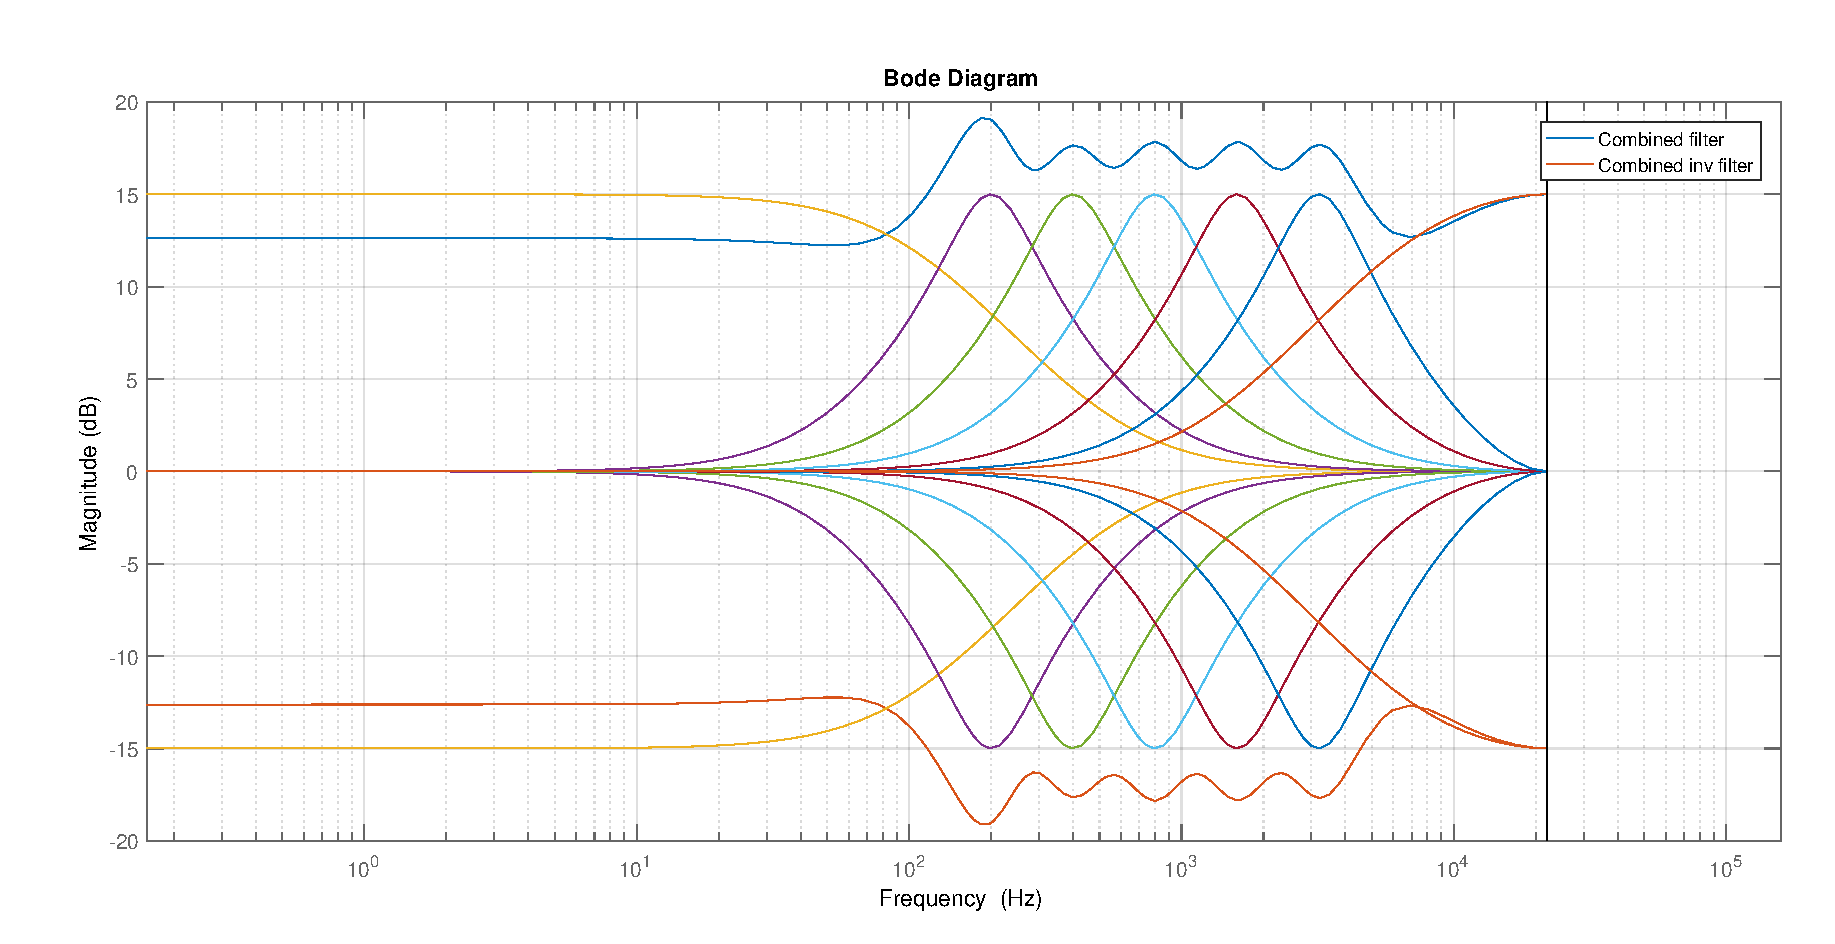
\includegraphics[width=\textwidth]{eq_z_domain_final.pdf}
        \caption{Bodeplot of the final equalizer's dynamic range in z-domain, with all bands fully amplified and fully attenuated.}
        \label{fig:eq_z_domain_final}
  \end{figure}
  
\subsection{Implementation of the equalizer}
When implementing the equalizer on the\gls{dsp} the amplifying part of the equalizer will be implemented first. This is because the amplifying part is the simplest one, since fewer coefficients have to be allocated in the \gls{dsp} memory. As seen in \autoref{eq:z_to_n7} the gain value, $G$, can be seen as an isolated scalar, which is multiplied on the coefficient fraction and a data value. Therefore e.g. $\frac{a_{peak1}}{b_{peak1}}$ can be written as a constant in the \gls{dsp}, no matter how much the specific band should amplify. This is not the case for the attenuating part of the equalizer, since the gain,$G$, is changing e.g. the coefficient $b_{peak1-cut}$, which is a denominator in \autoref{eq:z_to_n_peak_att}. 
The equalizer is implemented using 16-bits precision and the main algorithm of the amplifying part of the equalizer is shown in \autoref{code:eq_code}. 

\includeCode{equalizer.asm}{assembly}{61}{82}{The filter algorithm in the equalizer}{code:eq_code}{code/design/}

The code shows the implementation of one filter as for example the filter represented in \autoref{eq:z_to_n7}. Line 68 does the calculation $- \frac{b_{peak3}}{b_{peak1}} \cdot y_{peak}[n-2]$ and stores it in AC0. Line 69 does the calculation $-  \frac{b_{peak2}}{b_{peak1}} \cdot y_{peak}[n-1]$, adds it to what is already in AC0, and moves $y_{peak}[n-1]$ to $y_{peak}[n-2]$. This way the algorithm does the calculation of $y_{peak}[n]$. In line 74 $y_{peak}[n]$ is stored in $y_{peak}[n-1]$ to be ready to the next sample.  
Line 71 is special for the amplifying filters, because the coefficient in this line is zero, because \autoref{eq:z_to_n7} does not use $x[n-1]$ in its calculations. 
In \autoref{code:eq_code_parallel} the implementation of the block diagram in \autoref{fig:eq_parallel} is seen.

\includeCode{equalizer.asm}{assembly}{84}{118}{The implementation of \autoref{fig:eq_parallel}}{code:eq_code_parallel}{code/design/}

Line 117 is where all the outputs of the seven filters are added to the direct input.

%Raised Cosine

%The interference effects on the side lying bandpass filter can easily be avoided by using an digital equalizer with third-octave raised cosine characteristics. The difference between the  bandpass filter characteristics and the one with a raised-cosine are shown in \autoref{fig:raised_cosine_vs_traditional}
%
%\begin{figure} [htbp]
% \centering
%  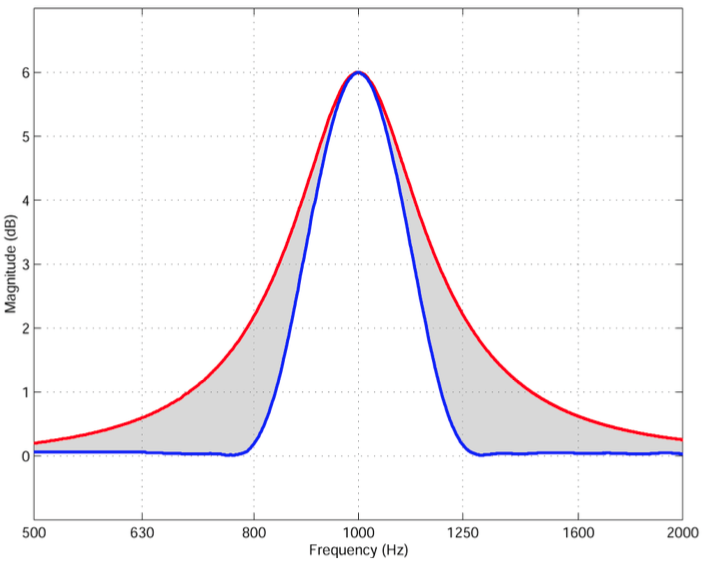
\includegraphics[width=0.7\textwidth]{raised_cosine_vs_traditional}
%  \caption{The photo shows the raised cosine bandpass filter characteristics versus traditional characteristics of third-octave bandpass filter \citep{nordic}
%  }
%  \label{fig:raised_cosine_vs_traditional}
%\end{figure}
%
%
%
%When using third-octave raised cosine bandpass filter, it is possible to make an equalizer where neighboring filters do not interfere with each other, or explained i another way, they interfere the right way, because a raised cosine filter does not leak into other third-octave bands like the traditional filter does. With this kind of filter it is possible to make a perfectly flat frequency response, and it is very close to an ideal equalizer. The \autoref{fig:raised_cosine_respond} shows the frequency response of a third-octave raised cosine equalizer designed by Dolby lake with the same gain and frequency settings as the analog equalizer at \autoref{fig:analog_equalizer}.
%
%\begin{figure} [htbp]
% \centering
%  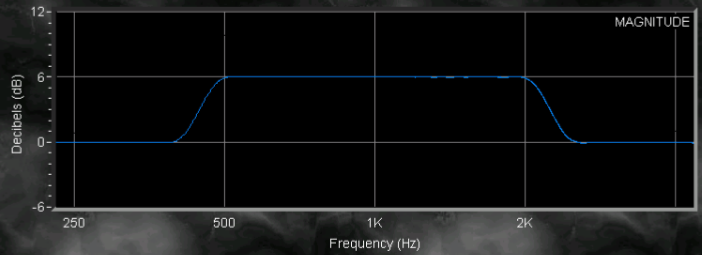
\includegraphics[width=0.8\textwidth]{raised_cosine_respond}
%  \caption{The photo shows an third-octave raised cosine equalizer frequency response  \citep{nordic}
%  }
%  \label{fig:raised_cosine_respond}
%\end{figure}
%
%
%The equalizer is used to compensate for the changes in sound due to different room characteristics, because the sound can be completely different in different rooms. The room characteristics will or can amplify or attenuate some frequency, and therefore the equalizer is very important to adjust the frequency in every new room.\citep{howtogeek} 
